\documentclass[10pt]{beamer}
\usepackage[slovene]{babel}
\usepackage[utf8]{inputenc}
\usepackage[T1]{fontenc}
\usepackage{lmodern}
\usepackage{mathptmx}
\usepackage{helvet}
\usepackage{courier}
\usepackage{hyperref}
\usepackage{wrapfig}
\usepackage{tikz}
\usepackage{tcolorbox}

\usetheme{CambridgeUS}

\begin{document}

\title[Finančni instrumenti osnovani na razpršenosti]{Finančni instrumenti osnovani na razpršenosti}
\author{Žan Jarc\\Mentorica: prof. dr. Damjana Kokol Bukovšek\\ Somentor: dr. Aleš Toman}
\institute [FMF]{ Fakulteta za matematiko in fiziko}

\begin{frame}
	\titlepage
\end {frame}

\begin{frame}
\textbf{Vsebina predstavitve}:
	\begin{itemize}
		\item Volatilnost trga
		\item Indeks Standard \& Poor’s 500 
		\item Indeks VIX
		\item VIX terminski posli (futures) in VIX opcije (options)
			\begin{itemize}
				\item VIX terminski posli
				\item VIX opcije
			\end{itemize}
	\end{itemize}
\end {frame}

\begin{frame}
\frametitle{Volatilnost trga}
\begin{itemize}
\item \textbf{Volatilnost trga} je volatilnost donosov finančnih instrumentov/naložb.

\item Volatilnost nam implicira razlike v donosih.

\item Če se trg strmo dviga/pada bo volatilnost visoka.
\item Govorimo lahko o dejanski volatilnosti (actual volatility) ali o teoretični volatilnosti (implied volatility).
\end{itemize}
\end{frame}

\begin{frame}
\frametitle{Indeks Standard \& Poor’s 500}
\begin{itemize}
\item \textbf{Indeks Standard \& Poor’s 500} ali \textbf{indeks S\&P 500} je najbolj uporabljena referenčna vrednost za splošen ameriški delniški trg.
\item Je kapitalizacijsko utežen indeks. 
\item Pri računanju indeska se upošteva cene delnic 500 največjih ameriških podjetij in število delnic posamenznega podjetja, ki so na voljo na odprtem trgu.
\item Indeks zasledimo pod kratico (ticker) SPX.

\end{itemize}
\end{frame}

\begin{frame}
\frametitle{SPX med letoma 2004 in 2019}
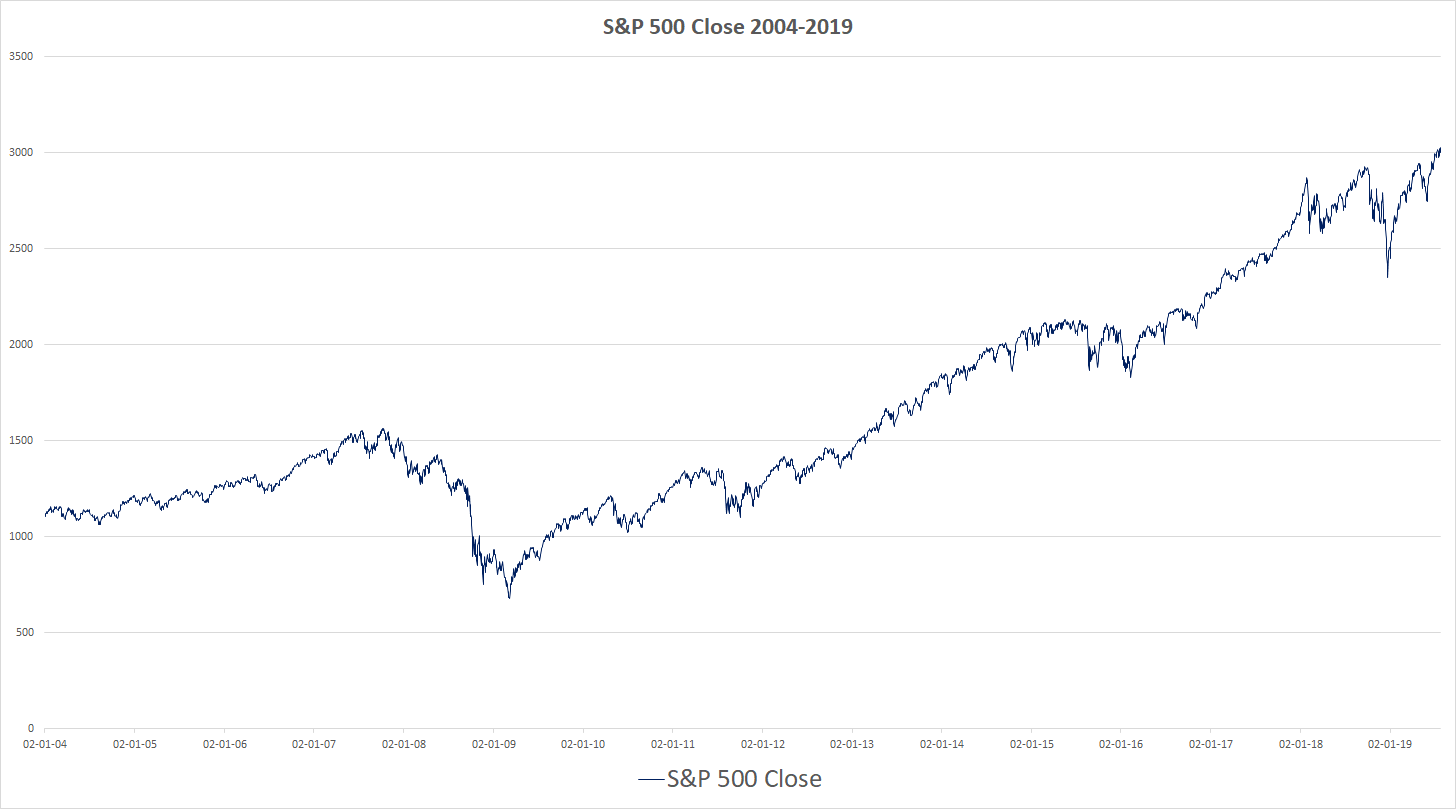
\includegraphics[width=1\textwidth]{./Grafi/SPX 2004-2019.png}
\end{frame}

\begin{frame}
\frametitle{SPX 2019}
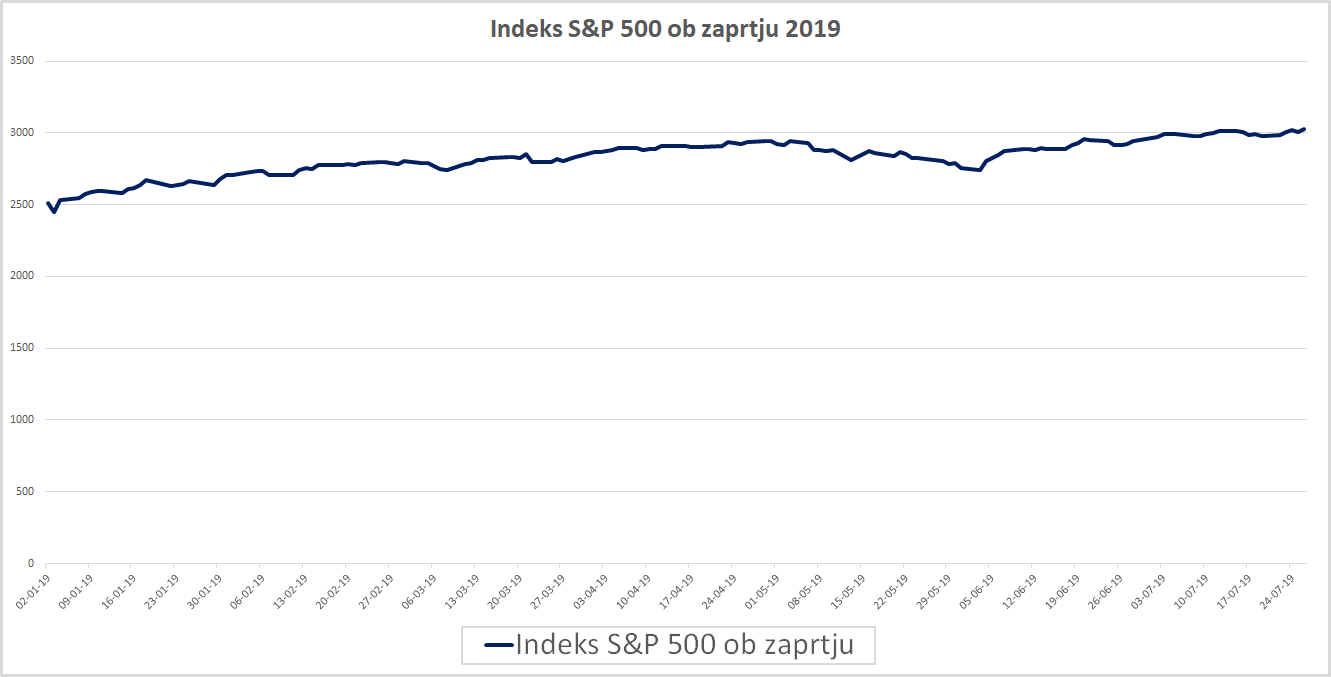
\includegraphics[width=1\textwidth]{./Grafi/SPX 2019.png}
\end{frame}

\begin{frame}
\frametitle{Indeks volatilnosti}
\begin{itemize}
\item Indeks \textbf{Cboe Volatility Index} ali \textbf{VIX} je bil razvit za napovedovanje pričakovane volatilnosti.
\item Indeks prikazuje 30 dnevno pričakovano volatilnost nakupnih in prodajnih opcij S\&P 500, ki se ne izplačajo (out-of-the-money), ki se zapadejo čez več kot 23 in manj kot 37 dni. 
\item Odraža pričakovanje trga, kako bo trg nihal v prihodnjih 30 dneh.
\item Omenja se ga tudi pod imenom indeks strahu (fear index).
\end{itemize}
\end{frame}

\begin{frame}
\frametitle{VIX in SPX primerjava}
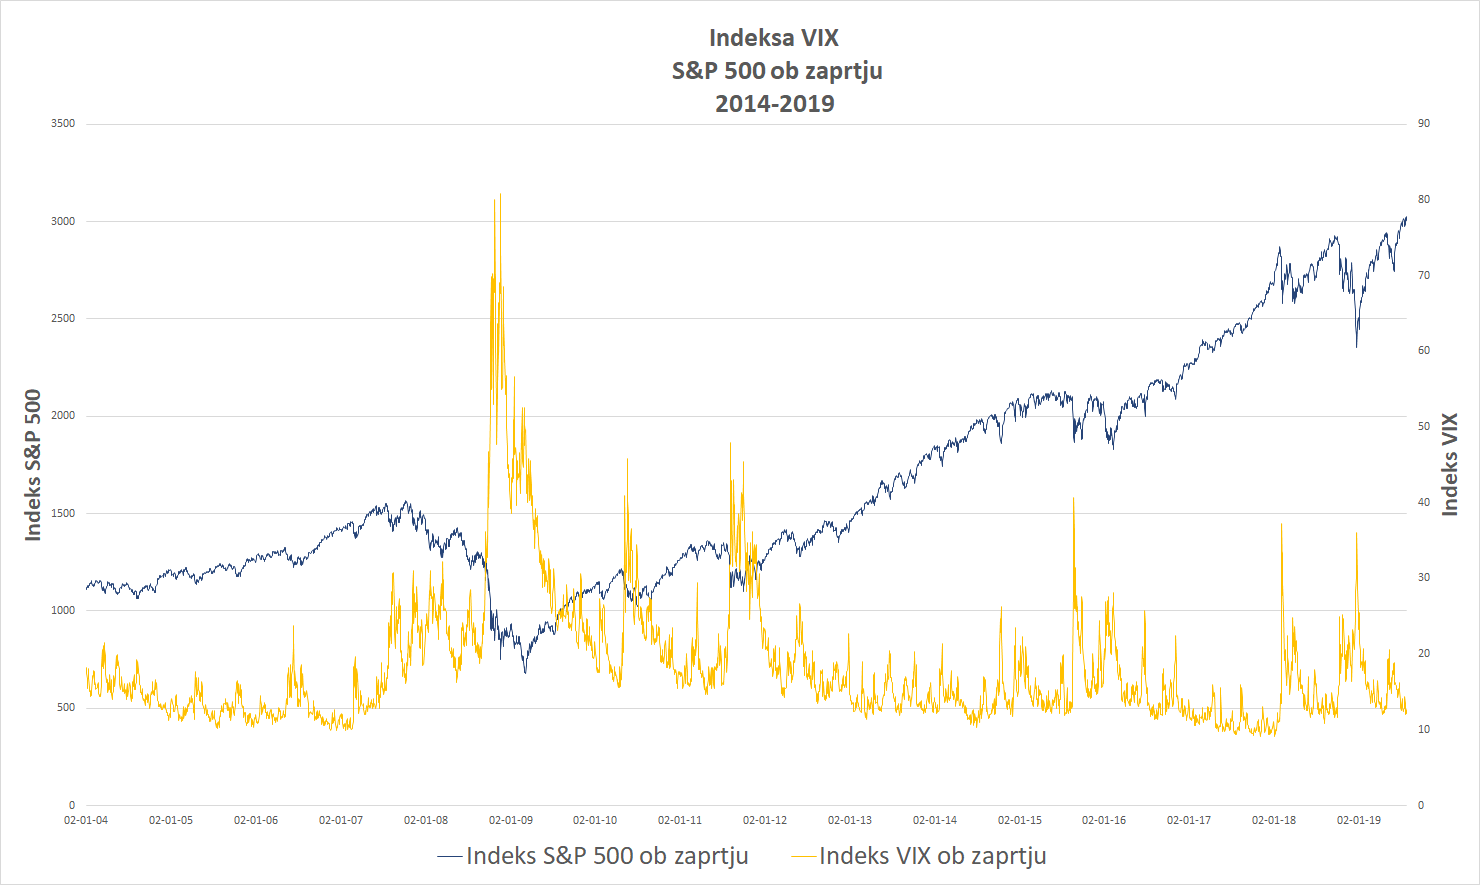
\includegraphics[width=1\textwidth]{./Grafi/VIX vs SPX 2004-2019.png}
\end{frame}

\begin{frame}
\frametitle{Lastnosti VIX}
\begin{itemize}
\item VIX in SPX sta negativno korelirana.
\item Negativna korelacija je najbolj vidna, ko finančni trgi doživijo velike izgube npr. za čas finančne krize med letoma 2008 in 2009. 
\item SPX je oktobra 2007 dosegel 1565,15 točk, najnižjo vrednost pa je dosegel marca 2009, ko je bila vrednosti 676,53. 
\item V istem časovnem okvirju je VIX zrasel iz 16,12 na 49,68 točke (vrh je dosegel novembra 2008 z vrednostjo 80,86). 
\item Ker je VIX le merilo volatilnosti trga, vanj ne moremo investirati.
\item Zato obstajajo različni finančni inštrumenti, katerih izplačila so odvisna od vrednosti VIX indeksa, VIX terminski posli in VIX opcije.
\end{itemize}
\end{frame}

\begin{frame}
\frametitle{VIX terminski posli}
\begin{itemize}
\item VIX terminski posli so v uporabi že od leta 2004 in jih najdemo pod kratico VX in VX01 do VX53.
\item Terminski posli imajo ročnost na sredo, ki je 30 dni pred petkom, ko zapadejo SPX opcije.
\item Vrednost terminskega posla s časom konvergira k vrednosti VIX. Zaradi tega so kratkoročni terminski posli iztekli veliko bolj občutljivi na spremembe VIX, kot pa tisti z daljšo ročnostjo. Posli z daljšo ročnostjo imajo tudi višjo izročitveno ceno.
\item Če sklenemo dolgo pozicijo v terminskem poslu, ko je VIX nizek, pričakujemo, da se bo volatilnost trga povišala, sicer s to investicijo ustvarimo izgubo (contango). 
\item Ob primeru, da je volatilnost trga visoka, pa s sklenitvijo dolge pozicije v terminskem poslu menimo, da se bo volatilnost zmanjšala (backwardation). 
\end{itemize}
\end{frame}

\begin{frame}
\frametitle{VIX terminski posli 2018}
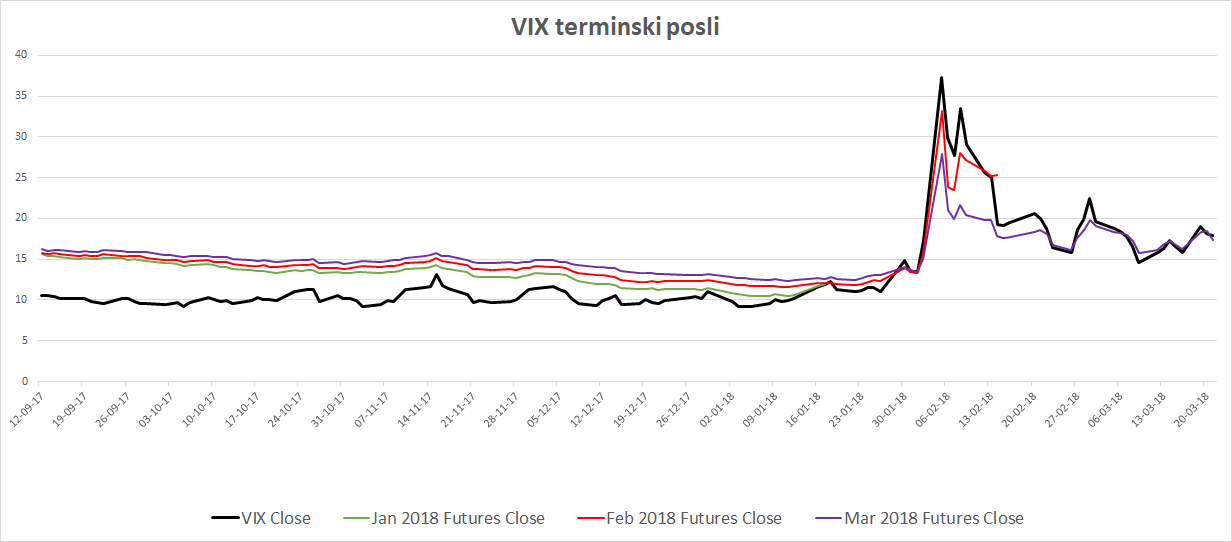
\includegraphics[width=1\textwidth]{./Grafi/VIX futures 2018.png}
\end{frame}

\begin{frame}
\frametitle{VIX opcije}
\begin{itemize}
\item VIX opcije so v uporabi od leta 2006 in jih najdemo pod kratico VIX.
\item Opcije so evropske.
\item Podobno kot terminski posli, imajo VIX opcije ročnost na sredo, ki je 30 dni pred petkom, ko zapadejo SPX opcije.
\item Vrednost opcij je vezana na VIX terminski posel z enako ročnostjo in ne na vrednost indeksa VIX.
\item S sklenitvijo nakupne VIX opcije se zavarujemo pred padcem vrednosti indeksa VIX.
\end{itemize}
\end{frame}

\end{document}


















\end{document}